\chapter{Descripción de la Misión}
el proyecto ha sido denominado lambda (lambda analyzes microorganisms biological damage in anomalous
 conditions), nombre que refleja el proposito general de la mision:
analizar los efectos de condiciones extremas como aceleraciones, vibraciones y variaciones
termicas sobre la integridad y viabilidad de microorganismos transportados a bordo del
cubesat.

en este captulo se describen las dos misiones que componen el proyecto lambda: la
mision primaria, de caracter obligatorio, que responde a los requerimientos mnimos establecidos por
la organizacion; y la mision secundaria, opcional y de libre eleccion, disenada con
un fuerte enfoque cientfico y desarrollada en colaboracion con el instituto de investigacion
medica mercedes y martn ferreyra (inimec-conicet-unc).

reconocemos el esfuerzo y dedicacion que implica la organizacion de esta competencia, as
como tambien el trabajo necesario para el diseno y construccion del cohete y su futuro lanzamiento.
por ello, consideramos que el vuelo del cubesat representa una valiosa oportunidad
que debe tener un proposito bien definido y significativo.

si bien ambas misiones son relevantes, el equipo ha dedicado especial atencion a la mision secundaria,
ya que permite una mayor libertad creativa e impulsa un enfoque original
orientado a la investigacion biomedica. en las siguientes secciones se detallan los objetivos,
fundamentos y enfoques tecnicos adoptados para cada una de las misiones que conforman el
proyecto lambda.

\section{Objetivos Misión Primaria}
La mision principal del presente proyecto consiste en registrar durante todo el vuelo del
CubeSat ciertas variables fsicas, las cuales son:

  \begin{itemize}
    \item Presion atmosferica,
    \item Temperatura ambiente,
    \item Aceleracion en los tres ejes,
    \item Angulo de giro en los tres ejes.
  \end{itemize}

Estas mediciones seran recopiladas, filtradas y almacenadas, y permitiran llevar a cabo
diversos analisis sobre el comportamiento del CubeSat durante su vuelo.
El objetivo sera aprovechar dichas mediciones para determinar el instante en el que se
alcanza el apogeo y su altitud maxima (valor de apogeo) respecto al punto de lanzamiento.
Por otro lado, tambien se determinara el tiempo total de ascenso y descenso, y se identificaran
las distintas fases del vuelo, tales como: inicio del ascenso, fin de la propulsion, el apogeo,

finalmente, la recuperacion.
Estas determinaciones, ademas de cumplir con los requisitos mnimos establecidos por la
organizacion de la competencia, seran de gran utilidad para la mision secundaria propuesta,
ya que permitiran interpretar correctamente los resultados obtenidos de la experimentacion
a realizar, que sera detallada en la siguiente seccion.

\section{Objetivos Misión Secundaria}
  \subsection{General}
    La mision secundaria del CubeSat, desarrollada en colaboracion con el Instituto de Investigacion
    Medica Mercedes y Martn Ferreyra (INIMEC-CONICET-UNC), se centra en
    el estudio de la viabilidad de celulas eucariotas, en particular el parasito Giardia Lamblia,
    expuestas a condiciones de estres fsico durante el lanzamiento y vuelo del vehculo portador. En
    este contexto, la viabilidad celular se define como la proporcion de celulas vivas y
    funcionales dentro de una poblacion sometida a factores adversos.
    Los principales factores de estres que se evaluaran incluyen las vibraciones mecanicas y
    las aceleraciones experimentadas durante el trayecto. Para ello, se analizaran varias muestras
    celulares dispuestas en condiciones experimentales distintas, con el objetivo de identificar
    posibles diferencias en sus respuestas fisiologicas.

    El sistema contara con control termico tanto para mantener la temperatura dentro de
    un rango adecuado para la preservacion celular, como para someter distintas muestras a
    distintas condiciones de temperatura. Posteriormente, se llevara a cabo un analisis postvuelo a
    fin de evaluar los efectos del entorno sobre cada muestra, mediante la observacion de
    cambios estructurales o alteraciones morfologicas en las celulas.

  \subsection{Giardia Lamblia}
    La Giardia Lamblia es un protozoario parasito flagelado que coloniza el intestino humano
    y animal, siendo una causa muy frecuente de enfermedad intestinal, contribuyendo a la carga
    de malnutricion en todo el mundo. La enfermedad producida por este parasito conocida
    como giardiasis es una parasitosis con gran importancia clnica y epidemiologica. Siendo esta
    la infeccion parasitaria del intestino humano mas frecuente de todo el mundo.

    Una caracterstica importante que poseen los microorganismos parasitos es su gran capacidad de
    adaptacion a los cambios del medio ambiente. La mayora de los parasitos ocupan
    diferentes nichos durante su travesa a por vectores y huespedes, desarrollando extraordinarios
    mecanismos de adaptacion que les permiten sobrevivir en condiciones que de otro modo
    los destruiran. Particularmente, Giardia Lamblia experimenta un proceso de diferenciacion
    a quiste, conocido como enquistamiento.

    El ciclo de vida simple de dos etapas de Giardia es central para su exito como parasito. Los
    quistes de Giardia Lamblia pueden sobrevivir en agua dulce fra durante meses, y se necesitan
    menos de 10 quistes para la infeccion humana. La exposicion de los quistes ingeridos al acido
    gástrico desencadena la exquistacion, una diferenciacion ropida y dramatica.

    Despues de la entrada en el intestino delgado, la pared del quiste se abre y emerge el
    parasito. Los trofozotos colonizan por debajo de la entrada del conducto biliar comun y pueden
    causar enfermedades, aunque no invaden. Si son transportados ro abajo, los trofozotos
    deben enquistarse para sobrevivir fuera del huesped. In vitro, Giardia se enquista en respuesta a
    los estmulos fisiologicos de aumento de bilis y pH ligeramente alcalino [2]. El estandar
    de oro para una enquistacion exitosa es la capacidad de los quistes para exquistarse.

    Otros parasitos intestinales importantes, como Entamoeba, Toxoplasma, Cryptosporidium, varias
    tenias y nematodos, se transmiten en forma de quistes u ooquistes. Sin embargo,
    el estudio de estos organismos se ve limitado por la imposibilidad de generar quistes maduros
    in vitro a diferencia de la Giardia Lamblia, por lo que se considera a este como un modelo
    de estudio para los demas parasitos.

    La via de enquistamiento de Giardia es un mecanismo clave de virulencia cuyo objetivo
    biologico es la diferenciacion hacia una forma que pueda sobrevivir en el ambiente e infectar
    a un nuevo huesped. El enquistamiento tambien promueve la evasion inmunitaria y es un
    objetivo para el desarrollo de vacunas y farmacos.

    La enquistacion es una transformacion gradual
    del trofozoto movil, flagelado, binucleado y con forma de media pera (Figura \ref{fig:enquistamiento}).
    Los trofozotos pierden su capacidad de fijacion a la pared intestinal; los fragmentos del disco de
    fijacion y los flagelos se internalizan. El metabolismo tambien disminuye a medida que las celulas
    se redondean y entran en latencia.

    \begin{figure}[H]
      \centering
      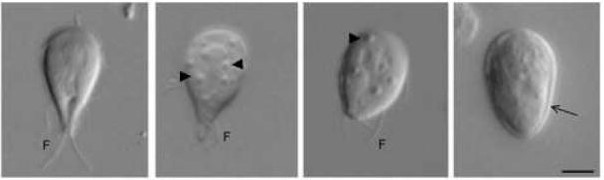
\includegraphics[width=1\textwidth]{./image/Giardia/Enquistamiento.jpg}
      \caption{Enquistamiento de \textit{Giardia Lamblia}: del trofozoíto al quiste. F, flagelos. Barra: 5 $\mu m$}
      \label{fig:enquistamiento}
    \end{figure}

    Las imagenes de izquierda a derecha muestran un trofozoto vegetativo, trofozotos despues de 21 y
    42 horas de enquistamiento y un quiste resistente al agua. [2]

  \subsection{Experimento}
    Se establecieron tres condiciones experimentales con el objetivo de evaluar el efecto de las
    variables asociadas al lanzamiento sobre el crecimiento y viabilidad de las muestras biologicas.
    Las condiciones disenadas son las siguientes:
 
    \begin{itemize}
      \item \textbf{Condición de vuelo (CUBESAT):} las muestras seran enviadas a bordo del CubeSat y
      sometidas a diferentes temperaturas: 10°C, 37°C (considerada óptima para el
      crecimiento) y 55C. Adicionalmente, se incluira una muestra sin control activo de temperatura,
      expuesta a las variaciones termicas propias del entorno.

      Todas las capsulas estaran posicionadas con una inclinacion de 45 con respecto al eje horizontal, condicion
      necesaria para favorecer la adherencia del parasito al medio de cultivo. Se busca analizar el
      impacto combinado de la microgravedad, las variaciones de presion, aceleraciones
      y la exposicion termica.

      \item \textbf{Condicion control terrestre (ESTACION TERRESTRE):} se replicara en tierra
      el mismo diseno experimental termico y la misma orientacion espacial de las capsulas
      que en el CubeSat. No obstante, las muestras permaneceran en un entorno terrestre
      controlado, sin estar expuestas a los factores propios del vuelo. Esta condicion permitira
      distinguir los efectos del lanzamiento de aquellos debidos a la condicion termica
      aplicada.

      \item \textbf{Condicion control optima (LABORATORIO):} se cultivara una muestra en condiciones optimas
      conocidas para el organismo en estudio: temperatura constante de
      37C, capsula inclinada a 45 y en ausencia de movimiento. Esta condicion constituye
      el control biologico para el experimento y servira como referencia para evaluar posibles
      desviaciones en las demas muestras.

      En todos los casos, se mantendran constantes el tipo de recipiente utilizado (capsulas de
      [material a definir]), el medio de cultivo y la cantidad inicial de trofozotos inoculados por
      capsula. Asimismo, tanto las muestras de las condiciones a) como b) seran sometidas al mismo
      proceso de traslado previo al inicio del experimento, con el fin de asegurar homogeneidad en
      las condiciones iniciales.
    \end{itemize}

  \subsection{Ensayos}
    Se realizaran ensayos a posteriori para evaluar si las condiciones a las cuales fue sometido afectaron la viabilidad o si las situaciones de estres disparan mecanismos clasicos de
    adaptacion de Giardia Lamblia, como por ejemplo; el enquistamiento, procesos de apoptosis,
    etcetera. Desarrollar que ensayos?

  \subsection{Procedimientos}
    Esta seccion describe los procedimientos necesarios para el cultivo y traslado de las muestras
    biologicas utilizadas en el experimento, manteniendo condiciones estandarizadas que
    aseguren su viabilidad y reproducibilidad.

    \subsubsection{Cultivo}
    Para cultivarlos axenicamente se utiliza medio TYI-S-33 (pH 7) suplementado con 10\% de
    suero bovino adulto y 5\% de bilis bovina (medio completo de crecimiento) (Diamond, Harlow
    un volumen determinado de medio. Los tubos se colocaron en gradillas orientadas con una
    inclinacion de aproximadamente $45\degree$, dentro de una estufa de cultivo a $37 \Celsius$.
    Luego de una hora, se comienza a observar la adhesion de los trofozotos a las paredes del
    tubo a traves de su disco ventral. De esta manera, se reproduce un entorno similar al que se
    encuentra in vivo, permitiendo la division de los trofozotos. A las 48 horas se obtiene una
    mono-capa de trofozotos en etapa de crecimiento. La inclinacion de las gradillas favorece
    una mayor superficie de adhesion sobre las paredes del tubo.

    \subsubsection{Traslado}
    Las condiciones optimas para el traslado consisten en mantener las muestras a $37\Celsius$ y con
    una inclinacion de $45\degree$. El tiempo de traslado puede extenderse hasta 48 horas sin que esto
    afecte significativamente las condiciones de crecimiento del parasito.

\section{Descripción del CubeSat}
En esta seccion se presenta una descripcion tecnica del CubeSat disenado para llevar a
cabo las misiones planteadas previamente. Se detallara como se planea abordar la implementacion de
los objetivos definidos, a traves de la integracion de subsistemas electronicos, mecanicos y de software.

Se incluyen diagramas de bloques que representan la arquitectura general del sistema y la
interaccion entre los distintos subsistemas, tales como adquisicion de datos, almacenamiento,
alimentacion electrica y control de sensores. Asimismo, se describen las herramientas de
calculo y simulacion empleadas durante las etapas de diseno y verificacion preliminar.

Tambien se presentan estimaciones iniciales de los presupuestos de masa, consumo de
potencia y volumen de datos, los cuales resultan fundamentales para validar la viabilidad del
sistema dentro de las restricciones impuestas por la competencia.

El desarrollo de esta seccion tiene por objetivo demostrar la coherencia tecnica entre los
requerimientos de mision y el diseno propuesto, as como documentar las decisiones adoptadas
durante el proceso de ingeniera del CubeSat.

  \subsection{General}
    En la Figura 5.2 se presenta el diagrama en bloques del sistema general desarrollado para
    el proyecto.
    El sistema general permite integrar la mision principal, enfocada en la recoleccion de
    parametros ambientales, con una mision secundaria orientada al control y documentacion de
    las condiciones de las muestras transportadas.

    \begin{figure}[H]
      \centering
      \resizebox{\textwidth}{!}{
      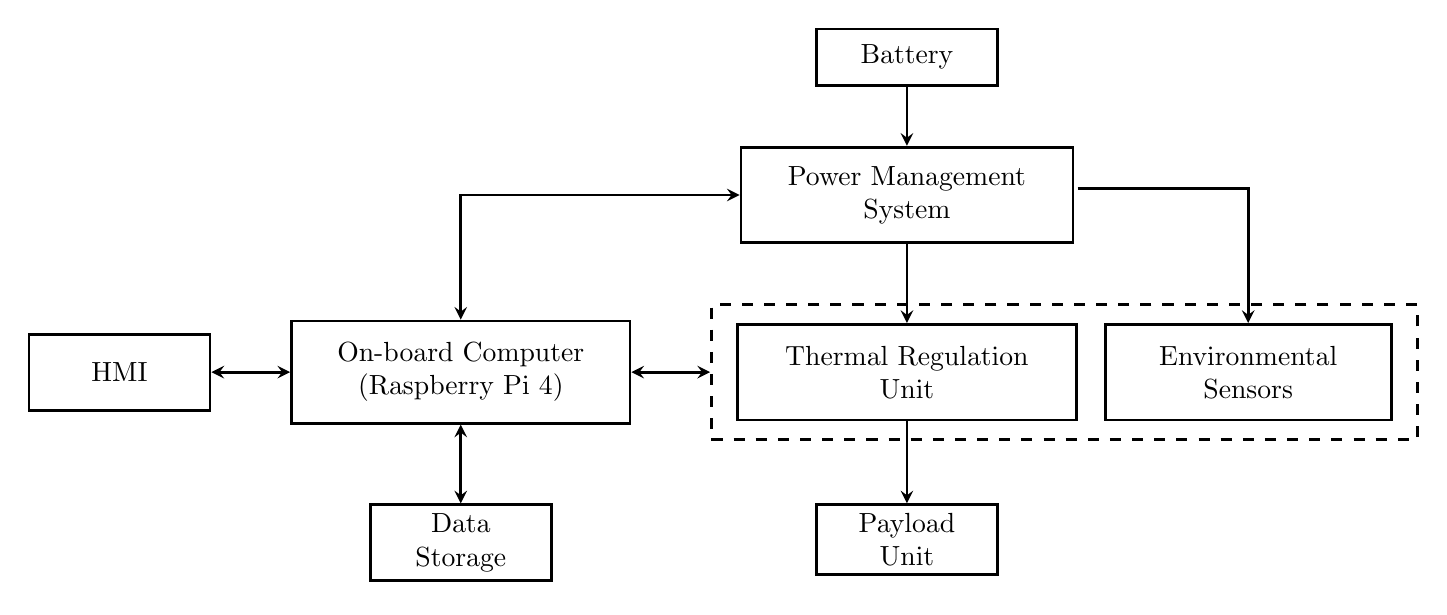
\begin{tikzpicture}
        % Paths, nodes and wires:
        \node[shape=rectangle, draw, line width=1pt, dash pattern={on 4pt off 4pt}, inner sep=0, minimum width=8.965cm, minimum height=1.715cm] at (11.833, 1.333){};
        \node[shape=rectangle, draw, line width=1pt, inner sep=0, minimum width=4.298cm, minimum height=1.215cm] at (9.833, 1.333){} node [anchor=center, align=center, text width=3.91cm, inner sep=5.5pt] at (9.833, 1.333){Thermal Regulation\\Unit};
        \node[shape=rectangle, draw, line width=1pt, inner sep=0, minimum width=3.631cm, minimum height=1.215cm] at (14.167, 1.333){} node [anchor=center, align=center, text width=3.243cm, inner sep=5.5pt] at (14.167, 1.333){Environmental Sensors};
        \node[shape=rectangle, draw, line width=1pt, inner sep=0, minimum width=2.298cm, minimum height=0.881cm] at (9.833, -0.792){} node [anchor=center, align=center, text width=1.91cm, inner sep=5.5pt] at (9.833, -0.792){Payload Unit};
        \node[shape=rectangle, draw, line width=1pt, inner sep=0, minimum width=2.298cm, minimum height=0.965cm] at (4.167, -0.833){} node [anchor=center, align=center, text width=1.91cm, inner sep=5.5pt] at (4.167, -0.833){Data Storage};
        \node[shape=rectangle, draw, line width=1pt, inner sep=0, minimum width=2.298cm, minimum height=0.715cm] at (9.833, 5.333){} node [anchor=center, align=center, text width=1.91cm, inner sep=5.5pt] at (9.833, 5.333){Battery};
        \node[shape=rectangle, draw, line width=1pt, inner sep=0, minimum width=4.298cm, minimum height=1.298cm] at (4.167, 1.333){} node [anchor=center, align=center, text width=3.91cm, inner sep=5.5pt] at (4.167, 1.333){On-board Computer\\(Raspberry Pi 4)};
        \node[shape=rectangle, draw, line width=1pt, inner sep=0, minimum width=4.215cm, minimum height=1.215cm] at (9.833, 3.583){} node [anchor=center, align=center, text width=3.827cm, inner sep=5.5pt] at (9.833, 3.583){Power Management\\System};
        \draw[stealth-stealth, line width=1pt] (4.167, 2) |- (7.708, 3.583);
        \draw[-stealth, line width=1pt] (12, 3.667) -| (14.167, 1.958);
        \draw[stealth-, line width=1pt] (9.833, 4.208) -- (9.833, 4.958);
        \draw[stealth-, line width=1pt] (9.833, 1.958) -- (9.833, 2.958);
        \draw[stealth-stealth, line width=1pt] (4.167, 0.667) -- (4.167, -0.333);
        \node[shape=rectangle, draw, line width=1pt, inner sep=0, minimum width=2.298cm, minimum height=0.965cm] at (-0.167, 1.333){} node [anchor=center, align=center, text width=1.91cm, inner sep=5.5pt] at (-0.167, 1.333){HMI};
        \draw[stealth-, line width=1pt] (9.833, -0.333) |- (9.833, 0.708);
        \draw[stealth-stealth, line width=1pt] (7.333, 1.333) -- (6.333, 1.333);
        \draw[stealth-stealth, line width=1pt] (1, 1.333) -- (2, 1.333);
      \end{tikzpicture}
      }
      \caption{Diagrama en bloques del sistema general}
      \label{fig:sistema_general}
    \end{figure}

  \subsection{Descripción de subsistemas}
    A continuacion, se describe la funcion de cada bloque y su interaccion dentro del sistema:
    \begin{itemize}
      \item \textbf{Battery:} Se emplearan seis bateras de polmero de litio (Li-Po) con una tension nominal de 3.7V
      y una capacidad individual de 3200mAh. Estas se organizaran en tres ramas
      conectadas en paralelo, cada una conformada por dos bateras en serie. Esta configuracion proporciona una tension total de 7.4V por rama (suma de dos bateras de 3.7V en
      serie) y una capacidad total de 71.04Wh, adecuada para satisfacer los requerimientos
      energeticos del CubeSat durante su operacion.

      \item \textbf{Power Management System (PMS):} es el subsistema responsable de administrar
      de forma segura y eficiente la energa proveniente de las bateras. Su funcion principal es
      distribuir la energa electrica a los distintos subsistemas del CubeSat, garantizando condiciones adecuadas de operacion, mediante el monitoreo, la proteccion y la regulacion.
      Especficamente, las funciones del PMS son:
      Proteger contra cortocircuitos o sobrecarga de corriente,
      Permite medir parametros electricos (como tension y corriente) y gestionar el
      encendido y apagado selectivo de distintos rieles de alimentacion lo que contribuye
      a una mejor eficiencia energetica y diagnostico en vuelo,
      Generar y estabilizar distintos niveles de tension requeridos por los subsistemas
      del CubeSat, como 3.3V para sensores, 5V para la computadora de abordo y 12V
      para cargas especficas.
      En definitiva, el PMS asegura que los requerimientos energeticos del CubeSat sean
      satisfechos de manera controlada, segura y adaptable durante toda la mision.

      \begin{figure}[H]
        \centering
        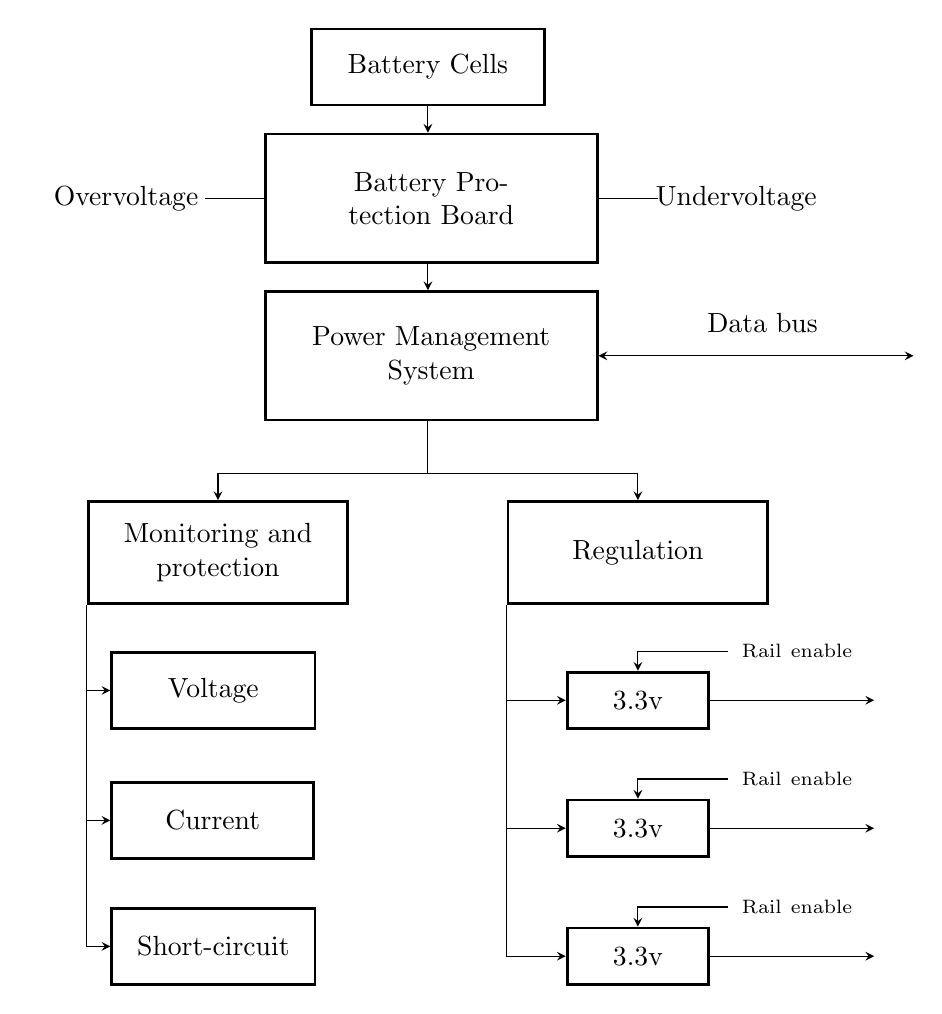
\begin{tikzpicture}
          % Paths, nodes and wires:
          \node[shape=rectangle, draw, line width=1pt, inner sep=0, minimum width=2.965cm, minimum height=0.965cm] at (8.833, 11.667){} node [anchor=center, align=center, text width=2.577cm, inner sep=5.5pt] at (8.833, 11.667){Battery Cells};
          \node[shape=rectangle, draw, line width=1pt, inner sep=0, minimum width=4.215cm, minimum height=1.631cm] at (8.875, 8){} node [anchor=center, align=center, text width=3.827cm, inner sep=5.5pt] at (8.875, 8){Power Management\\System};
          \node[shape=rectangle, draw, line width=1pt, inner sep=0, minimum width=4.215cm, minimum height=1.631cm] at (8.875, 10){} node [anchor=center, align=center, text width=3.827cm, inner sep=5.5pt] at (8.875, 10){Battery Protection Board};
          \node[shape=rectangle, inner sep=0, minimum width=2.5cm, minimum height=1cm] at (5, 10){} node [anchor=center, align=center, text width=2.147cm, inner sep=5pt] at (5, 10){Overvoltage};
          \node[shape=rectangle, draw, line width=1pt, inner sep=0, minimum width=3.298cm, minimum height=1.298cm] at (6.167, 5.5){} node [anchor=center, align=center, text width=2.91cm, inner sep=5.5pt] at (6.167, 5.5){Monitoring and\\protection\\};
          \node[shape=rectangle, draw, line width=1pt, inner sep=0, minimum width=1.798cm, minimum height=0.715cm] at (11.5, 3.625){} node [anchor=center, align=center, text width=1.41cm, inner sep=5.5pt] at (11.5, 3.625){3.3v};
          \node[shape=rectangle, draw, line width=1pt, inner sep=0, minimum width=3.298cm, minimum height=1.298cm] at (11.5, 5.5){} node [anchor=center, align=center, text width=2.91cm, inner sep=5.5pt] at (11.5, 5.5){Regulation\\};
          \node[shape=rectangle, draw, line width=1pt, inner sep=0, minimum width=2.581cm, minimum height=0.965cm] at (6.108, 0.5){} node [anchor=center, align=center, text width=2.193cm, inner sep=5.5pt] at (6.108, 0.5){Short-circuit};
          \draw[-stealth] (8.833, 7.167) -| (8.833, 6.5) -- (6.167, 6.5) -| (6.167, 6.167);
          \draw[-stealth] (8.833, 9.167) -| (8.833, 8.833);
          \draw[-stealth] (8.833, 11.167) -| (8.833, 10.833);
          \draw[-stealth] (12.417, 3.625) -- (14.5, 3.625);
          \draw[-stealth] (8.833, 6.5) -| (11.5, 6.167);
          \draw[stealth-stealth] (11, 8) -- (15, 8);
          \node[shape=rectangle, draw, line width=1pt, inner sep=0, minimum width=2.581cm, minimum height=0.965cm] at (6.108, 3.75){} node [anchor=center, align=center, text width=2.193cm, inner sep=5.5pt] at (6.108, 3.75){Voltage};
          \node[shape=rectangle, inner sep=0, minimum width=3.333cm, minimum height=0.667cm] at (13.083, 8.417){} node [anchor=center, align=center, text width=2.981cm, inner sep=5pt] at (13.083, 8.417){Data bus};
          \node[shape=rectangle, inner sep=0, minimum width=2.5cm, minimum height=1cm] at (12.75, 10){} node [anchor=center, align=center, text width=2.147cm, inner sep=5pt] at (12.75, 10){Undervoltage};
          \draw (6.75, 10) -- (6, 10);
          \draw (11, 10) -- (11.75, 10);
          \node[shape=rectangle, draw, line width=1pt, inner sep=0, minimum width=2.565cm, minimum height=0.965cm] at (6.1, 2.1){} node [anchor=center, align=center, text width=2.177cm, inner sep=5.5pt] at (6.1, 2.1){Current};
          \node[shape=rectangle, inner sep=0, minimum width=2.063cm, minimum height=0.5cm] at (13.671, 4.25){} node [anchor=west, align=left, text width=1.71cm, inner sep=5pt] at (12.639, 4.25){\scriptsize Rail enable};
          \draw[-stealth] (12.639, 4.25) -| (11.5, 4);
          \node[shape=rectangle, draw, line width=1pt, inner sep=0, minimum width=1.798cm, minimum height=0.715cm] at (11.5, 2){} node [anchor=center, align=center, text width=1.41cm, inner sep=5.5pt] at (11.5, 2){3.3v};
          \draw[-stealth] (12.417, 2) -- (14.5, 2);
          \node[shape=rectangle, inner sep=0, minimum width=2.063cm, minimum height=0.5cm] at (13.671, 2.625){} node [anchor=west, align=left, text width=1.71cm, inner sep=5pt] at (12.639, 2.625){\scriptsize Rail enable};
          \draw[-stealth] (12.639, 2.625) -| (11.5, 2.375);
          \node[shape=rectangle, draw, line width=1pt, inner sep=0, minimum width=1.798cm, minimum height=0.715cm] at (11.5, 0.375){} node [anchor=center, align=center, text width=1.41cm, inner sep=5.5pt] at (11.5, 0.375){3.3v};
          \draw[-stealth] (12.417, 0.375) -- (14.5, 0.375);
          \node[shape=rectangle, inner sep=0, minimum width=2.063cm, minimum height=0.5cm] at (13.671, 1){} node [anchor=west, align=left, text width=1.71cm, inner sep=5pt] at (12.639, 1){\scriptsize Rail enable};
          \draw[-stealth] (12.639, 1) -| (11.5, 0.75);
          \draw[-stealth] (9.833, 4.833) |- (10.583, 0.375);
          \draw[stealth-] (10.583, 2) -| (9.83, 1.996);
          \draw[stealth-] (10.583, 3.625) -| (9.835, 3.628);
          \draw[-stealth] (4.5, 4.833) |- (4.8, 0.5);
          \draw[stealth-] (4.8, 3.75) -| (4.498, 3.758);
          \draw[stealth-] (4.8, 2.1) -| (4.499, 2.107);
        \end{tikzpicture}
        \caption{Diagrama en bloques del subsistema Power Management System.}
        \label{fig:sistema_pms}
      \end{figure}

      \item \textbf{On-board Computer (OBC):} Tiene como funcion principal la gestion autonoma de
      la mision durante todo el vuelo. Esta unidad esta basada en una Raspberry Pi Zero 2
      W, equipada con el sistema operativo Raspberry Pi OS Lite, una version optimizada sin
      entorno grafico. Esta configuracion fue seleccionada por su bajo consumo energetico,
      reducido tamano y alta estabilidad operativa, cualidades esenciales para sistemas embarcados en entornos aeroespaciales.
      El proposito fundamental del OBC es tomar y almacenar el registro de los sensores,
      tales como aceleracion, orientacion, presion atmosferica y temperatura ambiente. Estas
      mediciones son gestionadas por el firmware, y almacenadas de forma estructurada
      facilitando su posterior lectura y procesamiento.

      El OBC tambien es responsable del control de subsistemas clave, como el de regulacion
      termica, utilizado para la mision secundaria mediante celdas Peltier, a traves del Sistema de
      administracion de energa (PMS). Ademas, mantiene una constante conexion
      con este sistema, actuando como intermediario entre el PMS y el HMI, lo que permite
      el monitoreo en tiempo real la integridad energetica de los distintos subsistemas. Entre
      el estado de carga de la batera.

      Una vez finalizado el vuelo, los archivos generados son relevados por el HMI, habilitando
      su analisis y visualizacion. Esta separacion entre adquisicion y procesamiento permite una asignacion
      eficiente de recursos, manteniendo al sistema embarcado centrado
      exclusivamente en tareas crticas durante la mision.

      A traves del HMI sera posible establecer el modo de operacion de la OBC. Teniendo los siguientes modos de operacion:
      \begin{itemize}
         \item \textbf{Apagado}
         \item \textbf{Pre Lanzamiento:} Inicializa los subsistemas y corrobora el correcto funcionamiento.
          Permite la conexion con la estacion terrena para su verificacion.
         \item \textbf{Lanzamiento:} Realiza solamente las rutinas crticas para el cumplimiento de la
        mision. Cortando cualquier va de comunicacion con la estacion terrestre.
         \item \textbf{Recuperacion de datos:} Rehabilita la comunicacion con la estacion terrestre
        permitiendo la visualizacion, analisis y descarga de datos.
         \item \textbf{Prueba:} Este modo sera utilizado durante le desarrollo del CubeSat permitiendo
        acceso administrativo al sistema.
      \end{itemize}

      \begin{figure}[H]
        \centering
        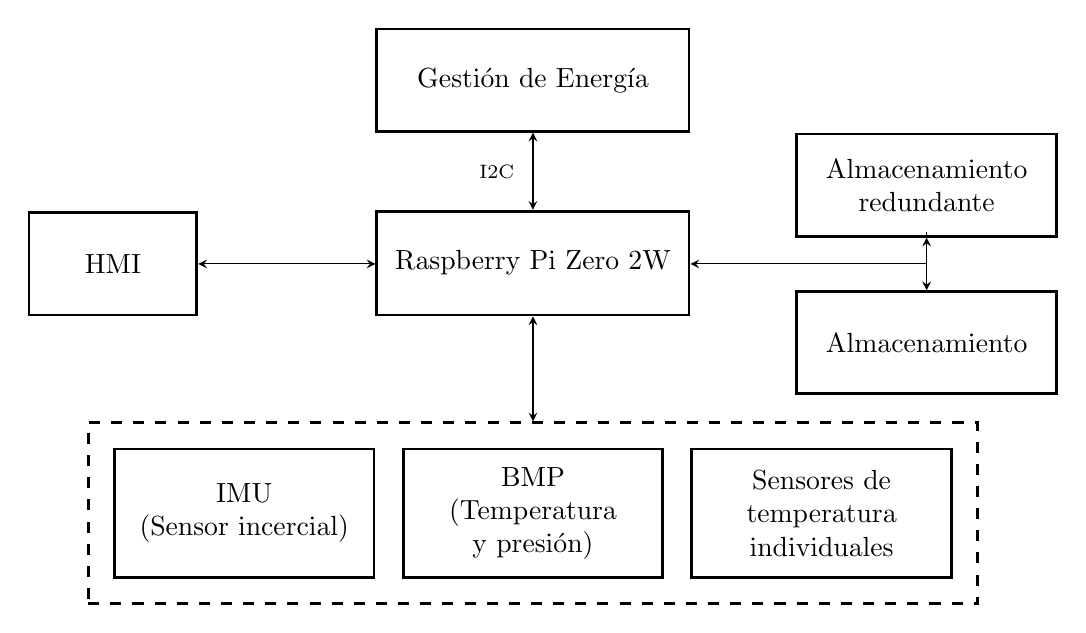
\begin{tikzpicture}
          % Paths, nodes and wires:
          \node[shape=rectangle, draw, line width=1pt, inner sep=0, minimum width=3.965cm, minimum height=1.319cm] at (9.667, 3.344){} node [anchor=center, align=center, text width=3.577cm, inner sep=5.5pt] at (9.667, 3.344){Raspberry Pi Zero 2W};
          \node[shape=rectangle, draw, line width=1pt, inner sep=0, minimum width=3.298cm, minimum height=1.631cm] at (6, 0.167){} node [anchor=center, align=center, text width=2.91cm, inner sep=5.5pt] at (6, 0.167){IMU\\(Sensor incercial)};
          \node[shape=rectangle, draw, line width=1pt, inner sep=0, minimum width=3.298cm, minimum height=1.298cm] at (14.667, 4.333){} node [anchor=center, align=center, text width=2.91cm, inner sep=5.5pt] at (14.667, 4.333){Almacenamiento redundante};
          \node[shape=rectangle, draw, line width=1pt, inner sep=0, minimum width=2.131cm, minimum height=1.298cm] at (4.333, 3.333){} node [anchor=center, align=center, text width=1.743cm, inner sep=5.5pt] at (4.333, 3.333){HMI};
          \node[shape=rectangle, draw, line width=1pt, inner sep=0, minimum width=3.298cm, minimum height=1.631cm] at (9.667, 0.167){} node [anchor=center, align=center, text width=2.91cm, inner sep=5.5pt] at (9.667, 0.167){BMP\\(Temperatura y presión)};
          \node[shape=rectangle, draw, line width=1pt, inner sep=0, minimum width=3.298cm, minimum height=1.631cm] at (13.333, 0.167){} node [anchor=center, align=center, text width=2.91cm, inner sep=5.5pt] at (13.333, 0.167){Sensores de temperatura individuales};
          \node[shape=rectangle, draw, line width=1pt, dash pattern={on 4pt off 4pt}, inner sep=0, minimum width=11.298cm, minimum height=2.298cm] at (9.667, 0.167){};
          \node[shape=rectangle, draw, line width=1pt, inner sep=0, minimum width=3.298cm, minimum height=1.298cm] at (14.667, 2.333){} node [anchor=center, align=center, text width=2.91cm, inner sep=5.5pt] at (14.667, 2.333){Almacenamiento};
          \node[shape=rectangle, draw, line width=1pt, inner sep=0, minimum width=3.965cm, minimum height=1.298cm] at (9.667, 5.667){} node [anchor=center, align=center, text width=3.577cm, inner sep=5.5pt] at (9.667, 5.667){Gestión de Energía};
          \node[shape=rectangle, inner sep=0, minimum width=0.917cm, minimum height=0.667cm] at (9.208, 4.5){} node [anchor=center, align=center, text width=0.564cm, inner sep=5pt] at (9.208, 4.5){\scriptsize I2C};
          \draw[stealth-stealth] (7.667, 3.333) -- (5.417, 3.333);
          \draw[stealth-stealth] (9.667, 4.021) -- (9.667, 5);
          \draw[stealth-stealth] (9.667, 2.667) -- (9.667, 1.333);
          \draw[stealth-] (11.667, 3.333) -- (14.667, 3.333);
          \draw[stealth-stealth] (14.667, 3.667) -| (14.667, 3);
        \end{tikzpicture}
        \caption{Diagrama de subsistema ”On-board Computer”}
        \label{fig:sistema_general}
      \end{figure}

      \item \textbf{Human-Machine Interface HMI:} Existen dos formas principales de interactuar con
        el CubeSat. La primera es mediante llaves de hardware que se conectan fsicamente al
        de interaccion es a traves de una interfaz web segura (HTTPS), accesible mediante una
        red local generada por la OBC.

        Adicionalmente, y reservadas exclusivamente para situaciones de emergencia, estaran
        habilitadas la conexion SSH (a traves de la misma red local) y la conexion UART
        mediante un puerto fsico. Esta ultima constituye la unica va de comunicacion que
        permanece activa durante todo el ciclo operativo del CubeSat.

        Desde la interfaz web, el usuario puede consultar variables crticas del sistema (temperatura, voltajes,
        corrientes, estado de sensores, entre otros), as como habilitar o
        deshabilitar subsistemas especficos, incluyendo rieles de alimentacion y modulos funcionales.
        Ademas de su rol operativo, la interfaz esta disenada tambien como una herramienta
        para el analisis post-mision. Una vez concluido el vuelo, permite la visualizacion, procesamiento
        y descarga de los archivos de datos registrados. Dicho procesamiento se realiza
        directamente en el cliente web, lo que reduce la carga sobre el sistema embarcado y
        permite un analisis dinamico sin necesidad de infraestructura adicional.

        En conjunto, el subsistema HMI proporciona una plataforma integral que centraliza el
        acceso a la informacion, optimiza la supervision tecnica y agiliza el analisis de resultados,
        facilitando as la validacion de los objetivos de la mision y la interpretacion de los
        fenomenos observados.

      \item \textbf{Data Storage:} La arquitectura de almacenamiento esta compuesta por dos tarjetas
        microSD de 16 GB: una como unidad principal, que aloja el sistema operativo y los
        datos primarios, y otra como unidad de respaldo, conectada mediante la interfaz SPI
        auxiliar. Ambas se encuentran configuradas en un esquema de RAID 1 por software,
        lo cual permite la replicacion sincronica de datos.

        En caso de fallos en la unidad principal
        como corrupcion logica o dano fsico, un conjunto de scripts de supervision ejecuta
        la des-conexion de la unidad afectada y procede a montar automaticamente el volumen
        redundante, asegurando as la continuidad operativa de la mision. Este mecanismo de
        conmutacion automatica simula un entorno de dual boot resiliente, adecuado para
        contextos de riesgo.

      \item \textbf{Environmental Sensors:} esta compuesto por los sensores encargados de medir los
        parametros fsico-ambientales durante el vuelo del CubeSat. Su funcion es proporcionar
        datos confiables y continuos que permitan cumplir con los objetivos establecidos en la
        mision principal, y sirvan de base contextual para interpretar los resultados de la mision
        secundaria.

        Este subsistema incluye los siguientes componentes:
        Unidad de Medicion Inercial (IMU - MPU9250): permite registrar la aceleracion en los
        tres ejes, as como los angulos de orientacion (roll, pitch y yaw) mediante acelerometros,

        Sensor barometrico BMP280: utilizado para medir la presion atmosferica en funcion
        del tiempo. Esta variable es clave para estimar la altitud relativa durante el ascenso,
        identificar el apogeo y complementar el analisis inercial con una referencia absoluta.

        Sensor de temperatura ambiente: mide la temperatura interna del satelite, proporcionando
        informacion crtica sobre el entorno termico durante el vuelo, tanto para la
        mision principal como para el monitoreo de las condiciones que afectan a los organismos
        involucrados en la mision secundaria.

        Los sensores seran gestionados directamente por el OBC, el cual se encargara de aplicar los
        filtros digitales necesarios para eliminar ruido, sincronizar temporalmente las
        muestras y almacenar la informacion.

        Este subsistema ha sido disenado bajo criterios de bajo consumo energetico, alta precision para
        los objetivos establecidos, y compatibilidad con sistemas embebidos basados
        en Raspberry Pi.

      \item \textbf{Thermal Regulation Unit (TRU):} tiene como objetivo controlar activamente la
        temperatura de distintas muestras biologicas durante el vuelo del CubeSat, en el contexto de la
        mision secundaria. Este sistema sirve para generar condiciones termicas
        especficas en los compartimientos que contienen los microorganismos.
        El sistema esta compuesto por los siguientes elementos principales:

      \begin{itemize}
        \item Celdas Peltier: dispositivos termoelectricos capaces de generar un gradiente de
          temperatura al aplicarles una diferencia de potencial. Su funcionamiento permite
          tanto calentar como enfriar las muestras, dependiendo de la polaridad y nivel de
          corriente aplicada. Se utilizaran tres celdas Peltier para mantener muestras en
          temperaturas distintas.

        \item Sensores de temperatura individuales: dispuestos en cada modulo termico, permiten medir la
          temperatura en contacto directo con las muestras, proporcionando
            una retroalimentación precisa al sistema de control.
      \end{itemize}

      El control de las celdas Peltier y la lectura de los sensores estara a cargo del OBC, que
      ajustara dinamicamente la potencia suministrada a cada celda a traves del PMS.

      \item \textbf{Payload Unit:}

    \end{itemize}

  \subsection{Herramientas de Calculo Empleadas}
    Para el desarrollo, simulacion y verificacion de cada uno de los subsistemas involucrados,
    se emplearan herramientas de calculo y software especficos que permitiran modelar los componentes
    y sus comportamientos, estimar el consumo de recursos, organizar la adquisicion y
    el procesamiento de datos, y validar el diseno general del sistema antes de su implementacion
    fsica.

    \begin{itemize}
      \item ANSYS Discovery (FEM)
      \item ANSYS Mechanical (FEM)
      \item Onshape (CAD)
      \item KiCad (CAD)
    \end{itemize}

  \subsection{Estructura}
    Para la estructura, tomamos inspiracion de un modelo disenado por EnduroSat [1]. El
    modelo esta caracterizado por el uso de estructuras fabricadas con laminas de aluminio
    plegadas, lo que le permite aprovechar al maximo el volumen del CubeSat, solo perdiendo
    dos veces el ancho de la lamina utilizada por cada eje.

    image/structure/render.png

    Figura 5.5: Renderizado de la estructura propuesta

    \subsubsection{Descripcion General}
      Como se menciono previamente, la estructura disenada emplea laminas de aluminio de
      2mm plegadas, para maximizar el volumen disponible, manteniendo una estructura que es
      rgida, facil de fabricar y manteniendo un modulo de cizalladura bajo debido a todos los
      puntos de fijacion disponibles. El CubeSat tambien dispone de ocho puntos de apoyo en
      las caras +Z y -Z (rieles), los cuales son fabricados por impresion 3D (FDM), utilizando
      Polipropileno como material, ya que no solo es liviano, si no que tambien es bastante ductil,
      y su adhesion entre capas es muy buena.

      Para el montaje de los componentes internos, la estructura integra cuatro varillas de
      acero lisas, las cuales serviran para evitar movimientos en los ejes X e Y, no obstante, no hay
      fijacion para el eje Z. Para evitar el movimiento de los diferentes subsistemas en el eje Z, es
      necesario ocupar todo el largo de las varillas.
      Los diferentes subsistemas se integran a la estructura en sus correspondientes carcasas,
      fabricadas con una impresora 3D, utilizando el Polipropileno como material, que tiene muy
      buenas propiedades de adhesion entre capas, permitiendo (en caso de ser necesario) crear
      volumenes que sean hermeticos.

    \subsubsection{Proceso de Integración}

      El armado del CubeSat, comienza con la colocacion de la tapa inferior (plano -Z) sobre
      el banco de armado, con los pliegues hacia arriba. A estos pliegues, se le colocan las cuatro
      esquinas, fijandolas con los tornillos y tuercas autobloqueantes. Una vez colocados las cuatro
      esquinas, se puede proceder a colocar las varillas en la cara interna de la tapa inferior (plano
      -Z), utilizando los tornillos correspondientes. Despues de haber colocado las varillas, se puede
      proceder a colocar los diferentes subsistemas uno por uno, conectandolos entre si. P1or ultimo,
      se coloca la tapa superior (plano +Z), se fijan las varillas con los tornillos, y utilizando la
      herramienta de ajuste disenada para acceder a las tuercas superiores, se colocan los tornillos
      con las tuercas autobloqueantes respetando el orden De esquina al centro.

    \subsubsection{Fabricación}

      La fabricacion del CubeSat es relativamente simple, ya que solamente se requiere una
      plancha de aluminio como materia prima para obtener el esqueleto basico del mismo. La
      plancha de aluminio requiere ser cortada previo al plegado, ya que estos cortes implementan
      geometras que no solo facilitan los pliegues, si no que en algunos casos los hacen posibles,
      agregando puntos de alivio. Ademas de los cortes, es necesario hacer las perforaciones necesarias y tambien los avellanados, ya que se puede dificultar hacerlos despues del plegado
      debido a la complejidad de la fijacion.
      Los cortes de las planchas de aluminio se van a realizar utilizando una CNC, y los pliegues
      con una plegadora de chapa.
      Las varillas seran cortadas, frenteadas, perforadas y roscadas (interna) utilizando herramientas manuales

    \subsubsection{Colocación de Muestras}

      La estructura del CubeSat permitira que las muestras se puedan colocar despues de
      finalizar el ensamblaje de la estructura. Esto se hace posible gracias a las aberturas de las
      tapas, de las cuales la del plano +Z, va a ser para acceder a una tapa en la carcasa que aloje
      el subsistema de carga util, y por donde se carguen las muestras a analizar. Esta tapa va a
      ser fijada con la tornilleria correspondiente

  \subsection{Criterios de Margenes}
    Para en analisis de presupuestos preliminares establecimos los margenes considerando las
    condiciones mas desfavorables

  \subsection{Presupuesto Preliminar de Masa}

  \subsection{Presupuesto Preliminar de Potencia}
    El presupuesto de potencia se calculo considerando el caso mas desfavorable en cada uno
    de los componentes.

    \begin{table}[H]
    \centering
    \resizebox{\textwidth}{!}{
    \begin{tabular}{|l|c|c|c|c|c|c|}
    \hline
    \textbf{Componente} & \textbf{Cant.} & \textbf{Tensión [V]} & \textbf{Corriente [A]} & \textbf{Potencia [W]} & \textbf{Subtotal [W]} & \textbf{* [A]} \\
    \hline
    Raspberry Pi Zero 2 W & 1 & 5.0 & 0.26   & 1.30   & 1.30   & 0.35   \\
    Sensor BMP280         & 1 & 3.3 & 0.0007 & 0.0023 & 0.0023 & 0.0006 \\
    Sensor MPU9250        & 1 & 3.3 & 0.0039 & 0.0129 & 0.0129 & 0.0035 \\
    Celdas Peltier 4x4 cm & 3 & 12.0& 0.833  & 10.00  & 30.00  & 8.10   \\
    \hline
    \textbf{Total}        & – & –   & –      & –      & \textbf{31.3152} & \textbf{8.45 @ 3.7V} \\
    \hline
    \end{tabular}
    }
    \caption{Consumo de corriente y potencia de los componentes en el caso más desfavorable.}
    \label{tab:consumo_componentes}
    \end{table}

  \subsection{Presupuesto Preliminar de Datos}
    Durante el vuelo se generaran y almacenaran diversos tipos de datos relacionados tanto
    con la mision primaria como con la mision secundaria. A continuacion se detalla el presupuesto preliminar de almacenamiento de datos considerando un periodo de recoleccion de 4
    horas.
    Cada muestra registrada incluye el instante temporal y el valor medido del parametro, ocupando 4 bytes cada uno, lo que da un total de 8 bytes por muestra. Ademas, consideramos
    la mayor frecuencia de muestreo permitida por cada sensor.

    \begin{table}[H]
    \centering
    \begin{tabular}{|l|c|}
    \hline
    \textbf{Vector} & \textbf{Tamaño de muestra} \\
    \hline
    Tiempo & 4 bytes \\
    Valor  & 4 bytes \\
    \hline
    \textbf{Tamaño total} & \textbf{8 bytes} \\
    \hline
    \end{tabular}
    \caption{Tamaño total fijo por muestra de cada parámetro}
    \label{tab:tamanio_muestra}
    \end{table}

    \begin{itemize}

      \item \textbf{Variables fisicas y ambientales}

      \begin{table}[H]
      \centering
      \begin{tabular}{|l|c|c|c|c|}
      \hline
      \textbf{Parámetro} & \textbf{Tipo} & \textbf{Frecuencia [Hz]} & \textbf{Muestras/4h} & \textbf{Tamaño [MB]} \\
      \hline
      Presión               & float & 157   & 2,260,800  & $\approx$ 8.63     \\
      Temperatura ambiente  & float & 157   & 2,260,800  & $\approx$ 8.63     \\
      Aceleración           & float & 4000  & 5,760,000  & $\approx$ 219.73   \\
      Ángulo de giro        & float & 8000  & 11,520,000 & $\approx$ 439.45   \\
      \hline
      \textbf{Total estimado} & -    & -     & -         & $\boldsymbol{\approx 685.07}$ \\
      \hline
      \end{tabular}
      \caption{Volumen de datos total y de cada variable físico-ambiental}
      \label{tab:volumen_datos}
      \end{table}

      \item \textbf{Control de temperatura de de las muestras celulares}

      \begin{table}[H]
      \centering
      \begin{tabular}{|l|c|c|c|c|}
      \hline
      \textbf{Parámetro} & \textbf{Tipo} & \textbf{Frecuencia [Hz]} & \textbf{Muestras/4h} & \textbf{Tamaño [MB]} \\
      \hline
      Temperatura ideal de cultivo & float & 157 & 2,260,800 & $\approx$ 8.63 \\
      Temperatura menor            & float & 157 & 2,260,800 & $\approx$ 8.63 \\
      Temperatura mayor            & float & 157 & 2,260,800 & $\approx$ 8.63 \\
      Temperatura ambiente         & float & 157 & 2,260,800 & $\approx$ 8.63 \\
      \hline
      \textbf{Total estimado}      & -     & -   & -         & $\boldsymbol{\approx 34.52}$ \\
      \hline
      \end{tabular}
      \caption{Volumen de datos de los controles de temperatura de las muestras celulares}
      \label{tab:volumen_datos_temperatura}
      \end{table}

      \item \textbf{Información gravada previamente}

      \begin{table}[H]
      \centering
      \begin{tabular}{|l|c|c|}
      \hline
      \textbf{Software} & \textbf{Versión} & \textbf{Tamaño} \\
      \hline
      S.O. Raspberry Pi OS Lite (Debian 12.0 "bookworm") & - & $\approx$ 2.1~GB \\
      Python                   & 3 & $\approx$ 27.5~\textit{MB} \\
      Dependencias python      & 1 & $\approx$ 150~\textit{MB} \\
      logrotate                & 1 & $\approx$ 100~\textit{KB} \\
      chrony                   & 1 & $\approx$ 2~\textit{MB} \\
      \hline
      \textbf{Total estimado}  & - & $\boldsymbol{\approx 2.3~GB}$ \\
      \hline
      \end{tabular}
      \caption{Consumo de almacenamiento de los componentes}
      \label{tab:almacenamiento_componentes}
      \end{table}
  
    \end{itemize}

    \begin{table}[H]
    \centering
    \begin{tabular}{|l|c|}
    \hline
    \textbf{Apartado} & \textbf{Tamaño estimado [MB]} \\
    \hline
    Variables físicas              & 685.07 \\
    Back up Variables físicas      & 685.07 \\
    Temperaturas celulares         & 34.52  \\
    Back up Temperaturas celulares & 34.52  \\
    Información grabada previamente & 2355 \\
    \hline
    \textbf{Tamaño total}          & \textbf{3794.3} \\
    \hline
    \end{tabular}
    \caption{Tamaño total estimado}
    \label{tab:tamano_total_estimado}
    \end{table}

    Teniendo en cuenta todos los datos a ser almacenados, estimamos un volumen total de
    aproximadamente 3.7 GB

\section{Secuendia de Operación}

\section{Aseguramiento de Misión}

  \subsection{Análisis de Confiabilidad}
    Para el analisis de la confiabilidad de la estructura del CubeSat, se empleo el suite de
    herramientas de ANSYS, en su version educativa. El suite provee un extenso catalogo de
    herramientas de analisis y simulaciones y a su vez un amplio catalogo de materiales con
    todas sus propiedades. Para nuestro CubeSat, decidimos emplear los analisis modales, de
    vibraciones aleatorias y de estructura estatica, de los cuales obtuvimos metricas como la
    fatiga en diferentes puntos de la estructura, deformaciones dadas las condiciones de prueba
    y factor de seguridad para diferentes puntos.

    Para las simulaciones fue necesario elegir un material para cada elemento separado que
    forma parte de la estructura. En el Cuadro \ref{tab:materiales_empleados} se puede ver la
    lista de materiales empleados y algunas de sus propiedades importantes.

    \begin{table}[H]
    \centering
    \small % reduce un poco el tamaño de fuente para ajustar mejor
    \begin{tabular}{|p{2.2cm}|p{2.3cm}|p{2.3cm}|p{2.5cm}|p{2cm}|p{2.5cm}|}
    \hline
    \textbf{Material} & \centering\textbf{Módulo de elasticidad} & \centering\textbf{Límite Elástico} & \centering\textbf{Límite de Rotura} & \centering\textbf{Densidad} & \centering\textbf{Usado en} \tabularnewline
    \hline
    Aleación de Aluminio & \centering $71 \cdot 10^9\,Pa$ & \centering $280 \cdot 10^6\,Pa$ & \centering $310 \cdot 10^6\,Pa$ & \centering $2770\,kg/m^3$ & Tapas y Esquinas \tabularnewline
    \hline
    Acero 4140 & \centering $212.5 \cdot 10^9\,Pa$ & \centering $652.2 \cdot 10^6\,Pa$ & \centering $1015 \cdot 10^6\,Pa$ & \centering $7850\,kg/m^3$ & Tornillería y Varillas \tabularnewline
    \hline
    Polipropileno & \centering $1461 \cdot 10^6\,Pa$ & \centering $34.6 \cdot 10^6\,Pa$ & \centering $37.62 \cdot 10^6\,Pa$ & \centering $903.4\,kg/m^3$ & Rieles de Apoyo y carcasas \tabularnewline
    \hline
    \end{tabular}
    \caption{Lista de materiales empleados.}
    \label{tab:materiales_empleados}
    \end{table}

    Debido a que aun no esta completamente definido como sera la disposicion interna de
    cada subsistema del CubeSat, para las simulaciones colocamos objetos que tienen las mismas
    dimensiones y materiales de las carcasas de los subsistemas, pero solidos (rellenos) y ajustados
    para que tengan el peso necesario para que el CubeSat llegue al kilogramo.

    \subsubsection{Preparacion del modelo}

       El ensamblaje del CubeSat se exporta desde la plataforma de CAD online utilizada (Onshape) en formato
       STEP. De ahi, se importa la geometra a ANSYS Mechanical, el cual nos permite crear la seleccion
       y asignacion de los materiales, fijar superficies de contacto y
       establecer superficies de fijacion. Luego de importar la geometria, ANSYS Mechanical
       automaticamente genera la malla para su posterior uso en simulacion.
       Es importante mencionar que para las simulaciones, los
       tornillos y tuercas no estan siendo tomados en cuenta. Esto se debe a que la complejidad que le agrega
       a la malla, y la cantidad de nodos que son necesarios

       Figura 5.6: Geometria importada

       para poder incluir las 32 tuercas y los 40 tornillos a
       la malla y al analisis, excede los limites de la licencia
       educativa por la cual estamos haciendo uso del software. En la figura (5.7) se puede ver la
       malla generada.

       Figura 5.7: Malla generada automaticamente por ANSYS Mechanical.

    \subsubsection{Analisis Modal}

      Para poder proceder a las simulaciones de vibraciones aleatorias (workmanship) y analisis
      de integridad estructural, es necesario determinar las frecuencias modales del CubeSat. En
      el Cuadro \ref{tab:modos_obtenidos} se pueden ver las frecuencias modales encontradas desde 0Hz hasta 2200Hz.
      Modo

      \begin{table}[H]
      \centering
      \begin{tabular}{|c|c|c|c|c|c|c|}
      \hline
      \textbf{Modo}       & 1           & 2           & 3           & 4         & 5           & 6          \\
      \hline
      \textbf{Frecuencia} & $536{,}89\,Hz$ & $541{,}52\,Hz$ & $908{,}97\,Hz$ & $1253\,Hz$ & $1616{,}2\,Hz$ & $1624{,}1\,Hz$ \\
      \hline
      \end{tabular}
      \caption{Modos obtenidos.}
      \label{tab:modos_obtenidos}
      \end{table}

    \subsubsection{Analisis de Vibraciones Aleatorias}

    En este analisis, se sometio el CubeSat a la curva G2 /Hz recomendada por la competencia. Como
    ANSYS Mechanical ya tiene incorporado el mecanismo para conectar puntos por
    tramos rectos, la curva resultante tiene que pasar por los puntos especificados en el cuadro
    (5.9), generando una curva como la de la figura (5.8).


    Figura 5.8: Curva (interpolada) de aceleracion G.

    Esta curva se aplica a los tres ejes del CubeSat, lo que permite generar los siguientes
    analisis de estres y tension.

    %image/fem/ansys_cubesat-vibration_stress.png
    Figura 5.9: Analisis de Estres.

    %image/fem/ansys_cubesat-vibration_strain-x.png
    Figura 5.10: Analisis de Tension en el eje X.

    %image/fem/ansys_cubesat-vibration_strain-z.png
    Figura 5.11: Analisis de Tension en el eje Y. Figura 5.12: Analisis de Tension en el eje Z.

    Como se puede ver en la figura (5.9), para el analisis de Estres equivalente, el pico maximo
    es de 108  106 P a. Analizando con mas detalle, este punto se encuentra en la superficie de
    contacto de la tapa inferior y la varilla. Debido al limite de resolucion, este punto de alta
    presion puede ser una falla de simulacion, pero en caso de que no lo sea, sigue estando por
    debajo del limite de rotura del aluminio y del acero, por lo que no presenta un problema.

    \subsubsection{Analisis Estatico}

    Se espera que el CubeSat este sometido a una aceleraciones de hasta 20g en el sentido +z y hasta 1g en
    los sentidos x e y. Para las simulaciones, se utilizaron
    estos valores con un factor de 1.25x. Un detalle que cabe destacar, es que todas las deformaciones presentes
    %image/fem/ansys_cubesat-static_accelerat
    en estas simulaciones, estan amplificadas visualmente para facilitar la deteccion patrones y fallas en el
    diseno de la estructura, por lo tanto, es fundamental
    interpretar los resultados en funcion de las escalas de
    color y los valores numericos de los distintos analisis,
    y no tomar como referencia la magnitud visual de las
    Figura 5.13: Vector de aceleracion padeformaciones mostradas. Aclarado esto, se muestran
    ra la simulacion estatica.
    a continuacion las simulaciones realizadas.

    %image/fem/ansys_cubesat-static_stress.png
    Figura 5.14: Analisis de Fatiga.
    Figura 5.15: Analisis de Estres.
    %image/fem/ansys_cubesat-static_safety.png
    %image/fem/ansys_cubesat-static_deformation.png
    Figura 5.16: Analisis de factor de seguridad. Figura 5.17: Analisis de deformacion total.

    Como se observa en la figura 5.15, la tension
    maxima alcanzada en la estructura es de 19  106 , Pa, valor significativamente inferior al
    limite de rotura del material, lo que indica que no existe riesgo estructural bajo las
    condiciones de carga previstas para el lanzamiento. Asimismo, la figura 5.16 muestra que el factor
    de seguridad es uniforme en toda la estructura y alcanza un valor constante de 15, lo cual
    proporciona un amplio margen respecto a posibles fallos. Finalmente, segun la figura 5.17,
    la deformacion maxima experimentada por el CubeSat es de apenas 4, m, lo cual resulta
    despreciable frente a las tolerancias mecanicas del sistema.

    Concluimos entonces que nuestra propuesta de estructura es valida y soportara las condiciones de lanzamiento.

  \subsection{Análisis de Riesgos}
    En esta seccion se identifican posibles fallos asociados al funcionamiento de los subsistemas
    del CubeSat, con el objetivo de implementar estrategias de mitigacion que contribuyan a
    aumentar la confiabilidad y la seguridad del sistema en cada fase de la mision. Identificacion:

    \begin{longtable}{ | m{2.5cm} | m{3cm} | m{3cm} | m{6cm} | }
      \caption{Análisis de Riesgos} \label{tab:analisis_riesgos} \\
      \hline
      \textbf{Riesgo} & \textbf{Causa} & \textbf{Impacto} & \textbf{Mitigación} \\
      \hline
      \endfirsthead

      \hline
      \textbf{Riesgo} & \textbf{Causa} & \textbf{Impacto} & \textbf{Mitigación} \\
      \hline
      \endhead

      \hline
      \endfoot

      \hline
      \endlastfoot

      Rotura de cápsulas de muestras & Sobrecargas mecánicas o vibraciones excesivas & Pérdida parcial o total de las muestras biológicas & Diseño de porta-cápsulas amortiguadoras. Pruebas de vibración según estándar GEVS. Cierre redundante de las tapas. \\
      \hline
      Fallo del sistema de regulación térmica & Mal dimensionamiento de los elementos Peltier o fallo de controlador en vuelo. & Exposición de muestras a temperaturas fuera de rango. & Control de temperatura con sensores. Validación térmica en cámara climática. Modos de degradación segura que desactivan los elementos Peltier para reducir consumo. \\
      \hline
      Pérdida de datos por fallo de almacenamiento & Corrupción de tarjeta microSD o falla en conmutación RAID por script. & Pérdida parcial o total de registros de muestras. & Verificación periódica de integridad (checksum SHA-256). Script de conmutación automática probado en PDR. Redundancia de almacenamiento de datos críticos. \\
      \hline
      Fallo del suministro eléctrico & Sobrecarga de rieles, cortocircuito o desconexión no deseada. & Apagado de subsistemas. & Protección contra sobre-corriente y subtensión en PMS. Pruebas de ciclos de carga-descarga de batería. Rieles críticos alimentados desde canales independientes. \\
      \hline
      Mal funcionamiento de la imu o barómetro & Descalibración por choque mecánico o ruido eléctrico. & Imposibilidad de determinar fases de vuelo con precisión. & Pruebas previas en condiciones similares. \\
      \hline
      Contaminación o degradación de muestras biológicas & Fugas de medios de cultivo, exposición al ambiente. & Resultados experimentales no válidos, pérdida de muestras. & Sellado hermético de tubos. Uso de materiales biocompatibles. Control de humedad en bahía de muestras. Análisis de vacío. \\
      \hline
      Fallo de comunicación prelanzamiento y poslanzamiento  & Rotura de hardware por aterrizaje o vuelo. & Imposibilidad de monitoreo inmediato luego del lanzamiento. & Conexión por UART. \\
      \hline
    \end{longtable}

  \subsection{Ensayos}
    \subsubsection{Estructura}
    \subsubsection{Peso}
    \subsubsection{Centro de masa}
    Para determinar experimentalmente el centro de masa del satelite, colocamos una madera
    rectangular de espesor mnimo sobre una superficie plana de modo que el lado mas estrecho
    y largo se encuentre en contacto con la superficie. Arriba colocamos el CubeSat formando 4
    angulos rectos, es decir que las direcciones sus aristas sean paralelas y perpendiculares a la
    direccion de la madera. Deslizamos el satelite horizontalmente hasta encontrar un punto de
    equilibrio, esa sera la coordenada del centro de masa en ese eje. repetimos el procedimiento
    para los demas ejes y verificamos, en cada caso, que se encuentren a una distancia del centro
    geometrico de a lo sumo 10 mm.

    \subsubsection{Bateras}
    \begin{itemize}
      \item \textbf{Capacidad real:} este ensayo tiene como finalidad determinar la capacidad efectiva
      de la batera, comparandola con la especificacion nominal del fabricante. Para ello, se
      descargara la batera con una corriente constante conocida hasta alcanzar el voltaje
      mnimo especificado. Se registrara el tiempo total de descarga para calcular la capacidad en mAh. El resultado permitira verificar si la batera puede sostener la demanda
      energetica del sistema durante el tiempo requerido.

      \item \textbf{Medicion de voltaje y corriente durante carga y descarga:} Durante las fases de
      carga y descarga, se monitorearan de forma continua los valores de tension y corriente
      entregados por la batera. Esto permitira evaluar la estabilidad de la fuente frente a
      distintas condiciones de carga, as como detectar cadas de tension o comportamientos
      no deseados que puedan comprometer la operacion de los subsistemas.
    \end{itemize}

\section{Plan de Proyecto}

  \subsection{General}
    Para llevar a cabo la mision del CubeSat, se ha definido una estructura de trabajo que
    divide al equipo en diferentes grupos, cada uno con responsabilidades especficas. Esta division
    busca optimizar el desarrollo del proyecto mediante una organizacion eficiente de tareas y
    recursos humanos.
    \subsubsection{Organizacion del Equipo}
      \begin{itemize}
        \item \textbf{Project Manager (PM)}
          Coordinador general del proyecto, responsable de la planificacion y del funcionamiento
          sincronizado de todos los grupos y subsistemas.
          \begin{itemize}
            \item Cortesini Perez, Luciano Tomas
          \end{itemize}
        \item \textbf{Grupo Mecanico}
         Encargado del diseno estructural del satelite.
          \begin{itemize}
            \item Cortesini Perez, Luciano Tomas
            \item Palombo, Franco
          \end{itemize}
        \item \textbf{Grupo Electronica}
          Responsable del diseno, desarrollo y pruebas de los subsistemas electronicos, incluyendo
          potencia y sensores.
          \begin{itemize}
            \item Gil, Ignacio
            \item Prieto, Angelo
          \end{itemize}
          \item \textbf{Grupo Software}
          Encargado del desarrollo del software tanto embarcado como de recuperacion y procesamiento de datos.
          \begin{itemize}
            \item Adragna, Jimena Sofa
            \item Koroch, Matias Adolfo
            \item Montesinos, Dana Carolina
          \end{itemize}
        \item \textbf{Grupo de Divulgacion}
          A medida de que nos interiorizabamos mas con nuestra mision e interactuabamos con
          distintos profesionales, docentes e instituciones que nos brindaron su tiempo y conocimiento
          como equipo nos empezamos a preguntar, de que manera podemos utilizar
          nuestro proyecto para impactar el la sociedad?

          Es asi como nace el grupo de Divulgacion para darle respuesta a una inquietud que
          surgio fruto del desarrollo de este proyecto. Consideramos valioso compartir los trabajos
          que se llevan a cabo en nuestra facultad para visibilizar el trabajo academico, motivar
          a otros estudiantes, reconocer el valor de la investigacion cientfica como as tambien
          crear puentes entre la universidad y la sociedad. No solo buscamos cumplir con los
          objetivos tecnicos y cientficos de la mision, sino tambien inspirar y promover el interes
          por la ciencia en la comunidad de nuestra region.

          Es por esto que designamos un grupo encargado de documentar las distintas etapas
          del proyecto registrando con fotos y videos, generando informes y difundiendo hacia la
          comunidad por medio de distintas plataformas y redes sociales.

          La implementacion del plan de comunicacion se desarrollara en dos fases. En una primer
          instancia se evaluaran y estableceran los canales digitales y, para ellos, se crearan los
          distintos perfiles institucionales con una identidad unificada en un marco educativo
          y de divulgacion cientfica. Luego, el trabajo se basara en un proceso iterativo en el
          que se documentara sistematicamente, se editara y adaptara el material multimedia y
          calendario de publicacion programada, se realizaran las publicaciones pertinentes y se
          realizara un monitoreo y ajuste basado en la retroalimentacion de la comunidad.

          Estimamos no solo llegar a las personas sino tambien generar dialogo que sea fructfero
          tanto para los demas como para el equipo, debido a esto planeamos ademas adaptar el
          contenido segun los intereses del publico, reconocer sus contribuciones e incluir
          herramientas que nos faciliten esta comunicacion bidireccional como formatos interactivos
          de preguntas y respuestas, encuestas, sesiones en vivo, entre otras.
          Encargados de la documentacion y difusion en el proyecto.
          \begin{itemize}
            \item Adragna, Jimena Sofa
            \item Koroch, Matas Adolfo
            \item Montesinos, Dana Carolina
            \item Prieto, Angelo
          \end{itemize}
      \end{itemize}


  \subsection{Cronograma}
    Con el objetivo de garantizar una ejecucion ordenada, eficiente y dentro de los plazos
    establecidos, se elaboro un cronograma detallado para cada uno de los grupos de trabajo que
    contempla las diferentes tareas ha realizar junto con los diferentes fechas y plazos estipulados
    para cada una de ellas.

    Utilizamos una herramienta basada en diagramas Gantt de gestion estrategica para lograr
    visualizar con facilidad la secuencia logica de actividades, sus respectivas duraciones, y las
    dependencias entre tareas.

    Para el desarrollo de este proceso se tuvieron en cuenta distintas variables como las fechas
    lmites, los objetivos planteados, la disponibilidad de tiempo, los recursos economicos y el
    capital humano.

    \subsubsection{Grupo Mecanico}
    Para una visualizacion del cronograma, se remite al diagrama Gantt incluido en el anexo.
    \subsubsection{Grupo Electronica}
    Para una visualizacion del cronograma, se remite al diagrama Gantt incluido en el anexo,
    figura 7.10 y figura 7.11.
    \subsubsection{Grupo Software}
    Para una visualizacion del cronograma, se remite al diagrama Gantt incluido en el anexo,
    figura 7.12.

  \subsection{Costos}

    Cuadro 5.11: Costos
